

\documentclass{sig-alternate-05-2015}

% Include useful packages
\usepackage{graphicx}
\graphicspath{ {images/} }
\usepackage{float}
\usepackage{subfig}


\begin{document}

% Copyright
\setcopyright{acmcopyright}


\title{A Reimplementation of Online Tracking by Learning Discriminative Saliency Map with Convolutional Neural Network}

\numberofauthors{2} 
\author{
% You can go ahead and credit any number of authors here,
% e.g. one 'row of three' or two rows (consisting of one row of three
% and a second row of one, two or three).
%
% The command \alignauthor (no curly braces needed) should
% precede each author name, affiliation/snail-mail address and
% e-mail address. Additionally, tag each line of
% affiliation/address with \affaddr, and tag the
% e-mail address with \email.
%
% 1st. author
\alignauthor
Aaron Gonzales\\
       \email{gonza647@msu.edu}
% 2nd. author
\alignauthor
Steven MW Hoffman \\
       \email{hoffm470@msu.edu}
}
% There's nothing stopping you putting the seventh, eighth, etc.
% author on the opening page (as the 'third row') but we ask,
% for aesthetic reasons that you place these 'additional authors'
% in the \additional authors block, viz.
\date{25 March 2016}
% Just remember to make sure that the TOTAL number of authors
% is the number that will appear on the first page PLUS the
% number that will appear in the \additionalauthors section.

\maketitle

\begin{figure*}[t]
\centering
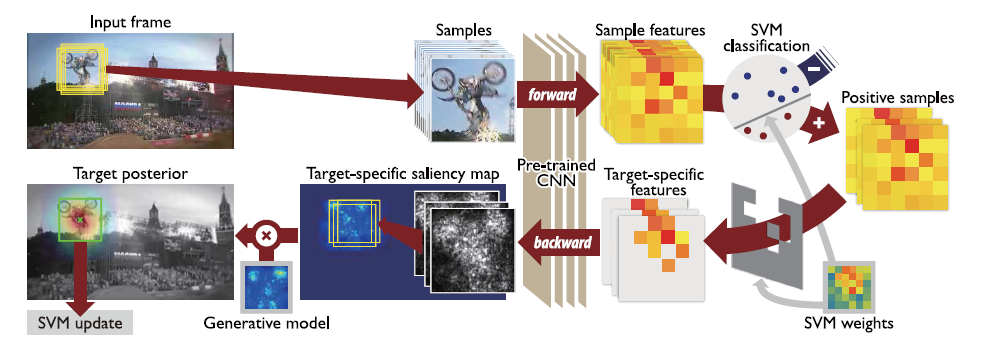
\includegraphics[width=\textwidth]{algorithm}
\caption{A pictoral description of the algorithm described by Hong, et al. in \cite{hong2015online}}
\label{fig:algor}
\end{figure*}

\section{Introduction}
We chose to implement our machine learning project with a \textit{deep learning thrust}.
We are basing our project on the work of Hong, et al. \cite{hong2015online}, and our goal is to reproduce their work through the creation of a viable demo.
Hong, et al. propose a novel online tracking scheme for use in applications where tracking an object through frames of a video is desired.
Although there are a large range of potential applications for object tracking software, it is still a difficult problem due to challenges of occlusion, pose variations, illumination changes, fast motion, and background clutter \cite{hong2015online}, and any potential tracking solution must have robust methods to overcome these challenges.
This paper proposes to solve these problems using the combined utility of both a convolutional neural network (CNN) and support vector machine (SVM), wherein a discriminative saliency map is produced and used to calculate the posterior probability of the target in the image.
The object tracking algortihgm by Hong, et al. is described below and is portrayed in Figure \ref{fig:algor}.

The tracking algorithm proposed by \cite{hong2015online} begins by first generating a set of sample images, each of which is drawn from candidate bounding boxes near where the target was located in the previous frame.
Each of these sample images is passed through a pre-trained CNN~\cite{jia2014caffe}.
A CNN is used because CNNs have been shown to be very successful at creating image representations useful for object discrimination.
Additionally, CNNs have shown promise in overcoming challenges from many of the current difficulties presented in object tracking, including pose variations, illumination changes, and background clutter.
For each image, the output from \textit{the first fully-connected layer} of the network is extracted and is used as the feature vector describing that image sample.
The image sample feature vector is then given to an SVM which will classify it as either a positive sample, including the object we are tracking, or a negative sample, which does not include the object we are tracking.
In contrast to the CNN, which is learned offline on generic image data not specific to the target, the SVM is learned online using the samples it has seen up to the previous video frame.
This allows the SVM to adapt to different types of objects which the user would like to track.
For each positive sample, the target-specific features are extracted by using those features which corresponded to positive weights in the SVM, setting all other feature values to zero.
The positive weights of the SVM are chosen because they are the weights which correspond to positively identifying a target.
These target-specific features are then backpropagated through the CNN, producing an image containing a saliency map.
A saliency map is created for every positive sample, and these are combined to make a final target-specific saliency map where larger values in the map indicate a larger posterior probability that the target is located at that pixel.
Through these means, the target can be segmented out of the image at a near pixel level.
With the target successfully segmented out of the frame, the algorithm begins anew in the next frame, creating candidate bounding boxes around where it found the target in the previous frame.

\section{Related Work}
The problem of object tracking in video is a large domain, so we will restrict our discussion here to a few works which also attempted to use CNNs to perform tracking, as these are most relevant to the paper we have chosen by Hong, et al. \cite{hong2015online}.
We also highlight how the approach proposed by Hong, et al. differs from these approaches, making it a novel work.

\cite{fan2010human} utilizes a CNN for tracking; however they use an offline trained CNN. They also require a separate class-specific network to track various other objects. Hong, et al \cite{hong2015online}, in contrast, proposes using a pre-trained CNN used for large scale image classification which is trained on generic image data. An online trained SVM is then used in conjunction with the CNN by Hong, et al. to learn the target specific information.

\cite{NIPS2013_5192} also uses a pre-trained network where a stacked denoising autoencoder is trained using a large number of images to learn generic image features. However, as this network is trained on small grey images, its representation power is limited.

\cite{7362006} proposed a target-specific CNN for tracking, where the CNN is trained online. However, this network is shallow in comparison with the deep CNN proposed by \cite{hong2015online}, and as such does not take advantage of the rich information a deep CNN provides.

In addition to the novelties described above, the tracking method proposed by \cite{hong2015online} differs from all three of the above papers in a few important ways.
First, it uses an online trained SVM with the offline trained CNN in order to adapt the tracking to whatever type of object the algorithm happens to be presented with.
Secondly, it uses saliency maps to find the precise location of the tracked object.

\begin{figure*}[t]
\centering
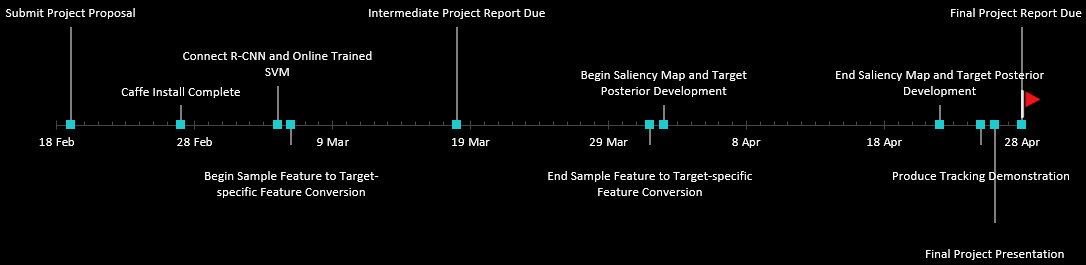
\includegraphics[width=\textwidth]{ProposedTimeline}
\caption{Our project milestones with tentative completion dates. Each tick-mark represents one day on the timeline.}
\label{fig:milestones}
\end{figure*}

\section{Data Description}
Following the form of Hong, et al.~\cite{hong2015online}, we expect to test the tracking algorithm against various benchmark sequences. 
There are a total of 50 tracking sequences which we have downloaded from a tracking benchmark dataset~\cite{wu2013online}.
These sequences present a variety of tracking challenges such as illumination variation, deformation, motion blur, background clutter, etc. 
In addition to these visual challenges, objects of interest vary from humans, to vehicles, to animals. 
Each of these sequences contain ground truth text files which contain bounding box information for objects of interest at each frame. 
Some of the videos contain multiple objects of interest and as a result come with multiple ground truth files. 
Depending on time availability we may decide to compare our implementation to that of Hong, et al.~\cite{hong2015online} and other top tracking implementations from the benchmark dataset.  Additionally, we may decide to test our implementation and report on our own select video sequences.

\section{Project Milestones}
As a reference the milestones presented in our project proposal are featured in Figure~\ref{fig:milestones}.
\subsection{Completed Milestones}

\subsubsection{Generating Candidate Sample Patches}
We have developed code that allows us to specify an initial bounding box around the starting object of interest. 
From each frame we are now able to generate target candidates by drawing 120 samples from a normal distribution defined by $x_i \sim \mathcal{N}(x_{t-1}^*,\sqrt{wh}/2)$, where $w$ and $h$ denote the width and height of the target bounding box. 
This is the same procedure as used by~\cite{hong2015online}.
These samples are then resized to 227 x 227 and used as input to our CNN.
An example of these samples is shown in Figure~\ref{fig:patches}.

\begin{figure}[h]
\centering
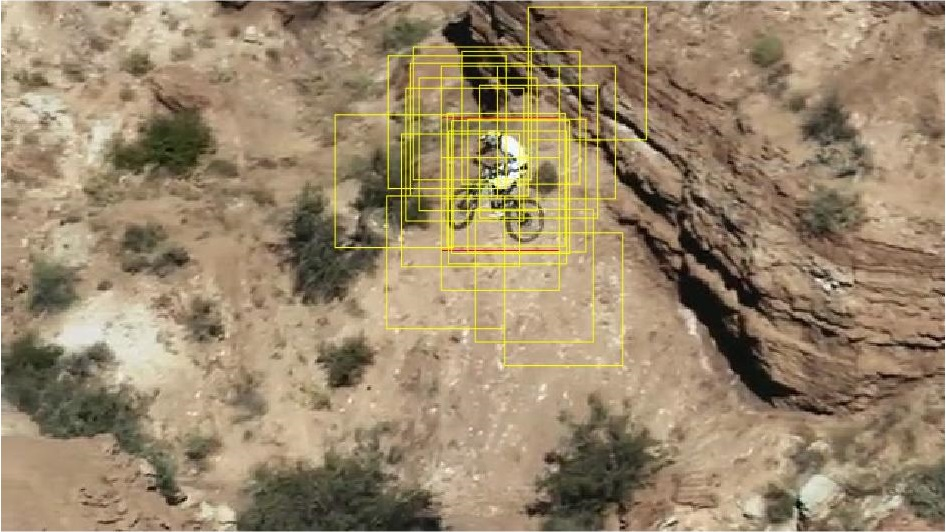
\includegraphics[width = 3in]{samples}
\caption{The bounding box (red) and the normally sampled candidate patches (yellow) for a biker from the video tracking dataset.}
\label{fig:patches}
\end{figure}

\subsubsection{Computing Sample Features with a CNN}
The original algorithm by Hong, et al.~\cite{hong2015online} used the Caffe Model Zoo implementation of the pretrained R-CNN created by Girshick, et al.~\cite{girshick2016region}.
The algorithm takes an image sample as an input and takes the output of the first fully connected layer of the R-CNN as the feature vector of the image sample.
However,~\cite{hong2015online} specified in their paper that CNN models other than Girshick's R-CNN may also be used for similar results.
Thus, to circumvent the large amount of time needed to install Caffe, we decided to instead use MatConvNet~\cite{vedaldi2015matconvnet}, a CNN toolkit for Matlab with a simple installation process.
MatConvNet provides several pretrained CNNs, and we decided to use VGG-F, a CNN that has achieved state-of-the-art performance on the ImageNet object recognition database~\cite{chatfield2014return}.
Upon acquiring this net, we wrote code that takes the network and the sample image as an input and returns the sample features of that image (i.e. the output of the first fully connected layer).

\subsubsection{Implementing an Online SVM}
Online SVM code has been acquired from Cauwenberghs, et al.~\cite{cauwenberghs2001incremental}. 
We may use different online SVM code in the future to match exactly what Hong, et al.~\cite{hong2015online} use in their approach, but for the moment, this code is sufficient. 
This code allows us to tweak various parameters to suite our needs, for example, whether or not to train the SVM incrementally and which kernel functions to use when training the SVM. 
While we have yet to connect the CNN and SVM, we have run tests on the SVM to help us better understand the manner in which to integrate our SVM, as well as to understand the results after training online and testing. 

\subsubsection{Computing Class Saliency Maps}
As one step of the algorithm, the target-specific features are back-propagated through the CNN in order to generate a target-specific saliency map, as detailed in~\cite{simonyan2013deep}.
This process involves taking the target-specific feature vector, inserting it into the first fully connected layer of the network, back-propagating this data to the input layer, and performing minor post-processing on this data.
Due to the process of back-propagation, the saliency maps are meant to highlight those pixels which have the most impact in identifying the  object in the image, effectively segmenting the foreground from the background.
A Matlab function was written to perform this operation.
Because the code to generate the target-specific features has not yet been written, this code currently takes as a parameter the sample features directly, which may include information about the background.
An example image with its corresponding saliency map is shown in Figure~\ref{fig:saliency}.
Note that the saliency map mostly highlights those pixels that correspond to the target foreground.

\begin{figure}[h]
\begin{tabular}{cc}
\subfloat[Original Image]{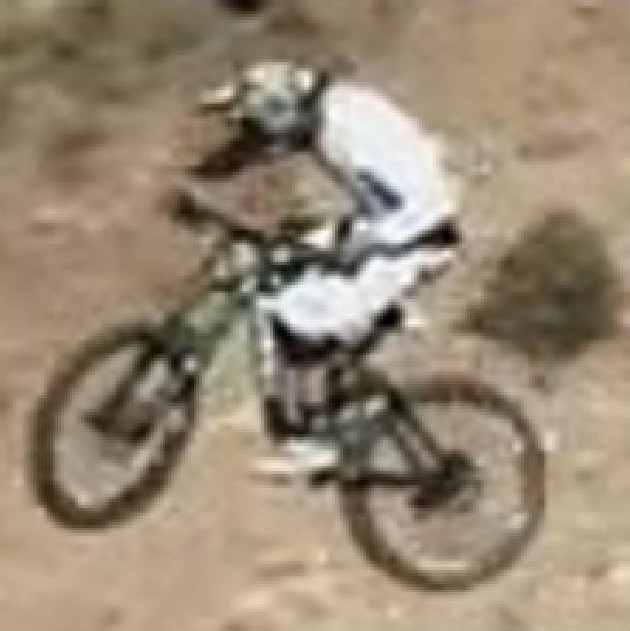
\includegraphics[width = 1.5in]{bike}}&
\subfloat[Saliency Map]{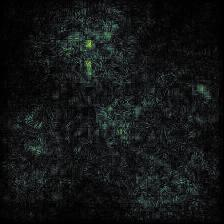
\includegraphics[width = 1.5in]{bike_saliency}}
\end{tabular}
\centering
\caption{The class saliency map for an image taken from the video tracking dataset used in this paper.}
\label{fig:saliency}
\end{figure}


\subsection{Remaining Milestones}
The connection of our CNN and SVM are not complete just yet. However, as we are now able to feed our CNN the appropriate input it is simply a matter of using the output of the first fully connected layer as input to our SVM. This process should be fairly straight forward, and thus we expect little issue connecting these two large components of our implementation. After connection we need to compute the SVM scores of candidate samples represented by the neural network features and classify them into target or background. Only samples with a positive SVM score will be used for developing the target-specific saliency map. We also need to implement the online training of the SVM after each frame, which may take a bit longer.

Although the class saliency maps have already been generated, a target-specific saliency map still needs to be generated by aggregating all the class saliency maps from a specific video frame.
We do not project that this will take very long to accomplish.
Then, in order to perform foreground-background segmentation, a generative model must be created and updated at each frame and convoluted with the target-specific saliency map. We are projecting that this task may take a substantial amount of our remaining time, as generating the model seems to be an intensive task.

After completing all the individual components of the algorithm, we will need to put them all together into one component, which we can iterate through frame by frame.
As this involves all the components previously worked on, it will likely take a few weeks to complete and debug.
Once having completed this, the remaining milestones will be to create a demo, record some results, create the final report, and create the final project presentation.
To create quality documents, this will also take several weeks to complete.

\bibliography{proj-proposal}
\bibliographystyle{unsrt}
\end{document}
